\documentclass[fleqn,11pt]{report}

\usepackage[utf8]{inputenc}
%\usepackage[russian]{babel}
\usepackage{textcomp}
\usepackage{booktabs} % For formal tables
\usepackage{amsmath}
\usepackage{natbib}
\usepackage{amssymb}
\usepackage[usenames,dvipsnames]{xcolor}
\usepackage{graphicx}
\usepackage{endnotes}
\usepackage{sectsty}
\usepackage[a4paper, margin=1.4in]{geometry}
\usepackage[hang,flushmargin]{footmisc}
\usepackage[font=small]{caption}
% \usepackage{tgtermes}
\usepackage[sfdefault,lf]{carlito}
%\usepackage{lmodern}
%\usepackage[scaled]{beramono}
\usepackage[scaled=0.8]{noto}
\usepackage[T1]{fontenc}

% \usepackage{caladea}
\usepackage[colorlinks]{hyperref} % [hidelinks]
\usepackage{hypcap}
\usepackage{fancyvrb}

\hypersetup{
linkcolor=Black,
citecolor=Mahogany,
filecolor=Black,
urlcolor=Blue,
menucolor=Black,
runcolor=Black
}
\renewcommand\enoteformat{%
  \raggedright
  \leftskip=1.8em
  \makebox[0pt][r]{\theenmark. \rule{0pt}{\dimexpr\ht\strutbox+}}%
}

\urlstyle{sf}

\widowpenalties 2 10000 0
\sectionfont{\large}
\chaptertitlefont{\LARGE}
%\renewcommand*\thesection{\arabic{section}}
%\setcounter{secnumdepth}{0} % sections are level 1

\newcommand{\kvd}[1]{\textnormal{\ttfamily\bfseries #1}}
\newcommand{\ident}[1]{\textnormal{\ttfamily #1}}

\begin{document}
\title{\Huge\textbf{Simple programming tools \\for data exploration}}
\author{Tomas Petricek}
\maketitle

\chapter*{Preface}
\label{ch:preface}
\addcontentsline{toc}{chapter}{\nameref{ch:preface}}

yo

\addcontentsline{toc}{chapter}{Contents}
\tableofcontents

\part{Commentary}

\chapter{Introduction}

The rise of big data, open government data initiatives \citep{attard-2015-opengov},\footnote{See
\url{https://data.gov} and \url{https://data.gov.uk}, but also \url{https://opendata.gov.cz} as
examples.} and civic data initiatives means that there is an increasing amount of raw data available
that can be used to understand the world we live in, while increasingly powerful machine learning
algorithms give us a way to gain insights from such data. At the same time, the general
public increasingly distrusts statistics \citep{davies-2017-statistics} and the belief that we
live in a post-truth era has become widely accepted over the last decade.

While there are complex socio-political reasons for this paradox, from a merely technical
perspective, the general public's lack of engagement with data-driven insights should perhaps
not be a surprise. We lack an accessible data exploration technologies that would allow
non-programmers such as data journalists, educators and data-literate citizens to explore complex
data and produce transparent data visualizations that can be understood, corrected and adapted by
a broad range of end-users.

The technology gap is illustrated in Figure~\ref{fig:gap}. On the one hand, graphical tools such as
spreadsheets are easy to use, but they are limited to small tabular data sets and are error-prone
\citep{panko-2015-errors} and do not aid transparency. On the other hand, programmatic tools for
data exploration such as Python and R can tackle complex problems, but require expert programming
skills for completing even the simplest tasks.

\begin{figure}[h!]
\centering
\vspace{0.5em}
  \caption{Illustration showing a gap between easy to use but limited spreadsheets
  and unlimited but hard to use programming tools. Adapted from \citet{edwards-2015-transcript}.}
\label{fig:gap}
\vspace{-0.5em}
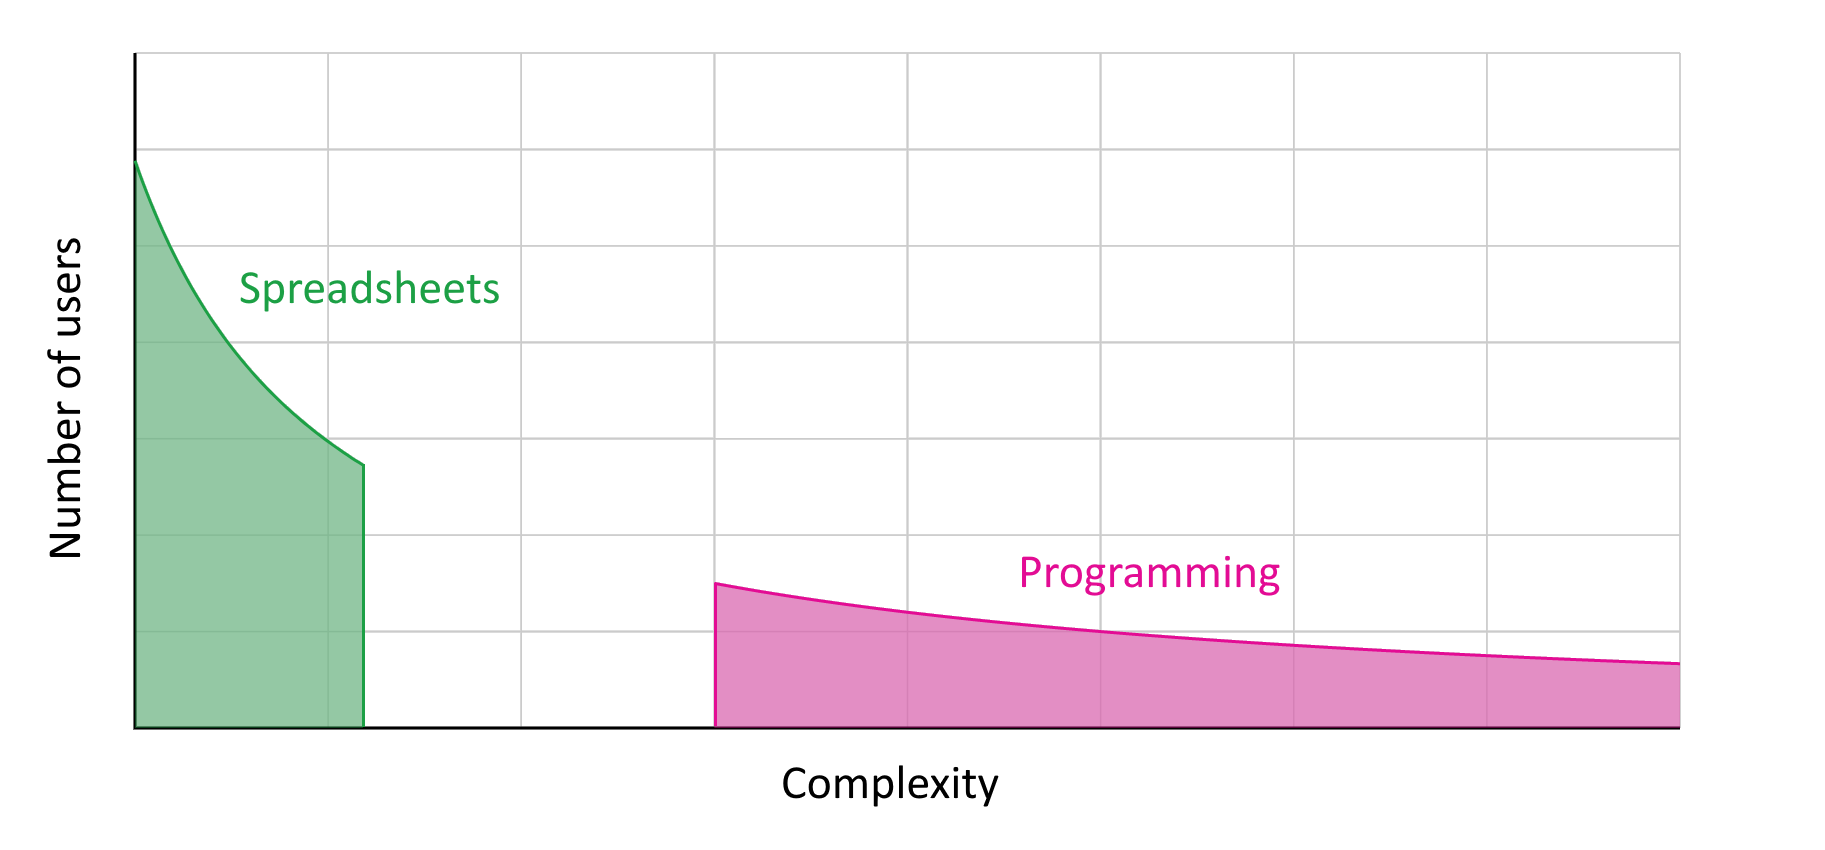
\includegraphics[scale=0.25]{img/gap.png}
\end{figure}

The above illustration should not be taken at face value. Although there is no single accepted
solution, there are multiple projects that exist in the gap between spreadsheets and programming
tools. However, the gap provides a useful perspective for positioning the contributions presented
in this thesis. They all attempt to fill or narrow the gap in some way. In particular, some
of the work develops novel tools that aim to combine the simplicity of spreadsheets
with the power of programming for the specific domain of data exploration. Some of the work
focuses on making regular programming with data easier, or making simple programming with data
accessible to a greater number of users.

\section{Requirements of simple tools for data exploration}

Although the tools and techniques presented in this thesis are more broadly applicable,
the focus of this thesis is on a particular kind of data exploration tools. I focus on tools
for data analysts who are technically skilled and information-literate, but are not programmers.
This includes data journalists, public servants and analysts at non-government organizations or
in the commercial sector. My work also focuses on the production of data analyses that are of
interest to a broader readership. The produced reports should be accessible not just to 
data analysts, but also to a broader non-technical public.
%
In the subsequent discussion, I distinguish between a \emph{data analyst}, who is a
technically skilled non-programmer and a \emph{reader}, who is interested in the results, but not
necessarily technical. This context leads to a number of requirements for the envisioned data
exploration tools:


\begin{itemize}
\item \emph{Gradual progression from simple to complex}. The system must allow non-experts with
limited resources to easily complete simple tasks in an interface that later allows them to
learn more and tackle more complex problems. In the technical dimensions of programming systems
framework \citep{jakubovic-2023-techdims}, this is known as the staged levels of complexity
approach to the learnability dimension.

\item \emph{Support transparency and openness}. The readers of the resulting data analyses must
be able to understand how the analysis was done and question what processing steps and parameters
have been used in order to critically engage with the problem.

\item \emph{Enable reproduction and learning by percolation}. A reader should be able to
redo steps through which a data exploration was conducted in order to reproduce the results, but
also to learn how to use the system. This is possible in the spreadsheet formula language
\citep{sarkar-2018-spreadsheets}, but not in the graphical interface.

\item \emph{Encourage meaningful reader interaction}. The reader should not be just a passive
consumer of the data analyses. They should be able to review and understand the analysis, but
also make simple modifications such as changing analysis or visualization parameters,
as is often done in interactive visualizations produced by journalists \citep{kennedy-2021-engagements}.
\end{itemize}

The above criteria point at the gap between spreadsheets and regular programming systems
illustrated by Figure~\ref{fig:gap} and there are multiple possible solutions and approaches to
satisfy the above criteria. This thesis explores one particular point in the design space,
which is to treat data exploration as a programming problem. I aim to show that a simple programming
tools for data exploration can satisfy the above criteria and make the production of
open and transparent data analyses accessible even to non-programmers.

\section{Data exploration as a programming problem}

Data exploration is typically done using a combination of tools including spreadsheets,
programming tools, online systems and ad-hoc utilities. Spreadsheets like Excel and business
intelligence tools like Tableau \citep{wesley-2011-tableau} are often used for manual data
editing, reshaping and visualization. More complex and automated data analyses are done in
programming languages like R and Python using a range of data processing libraries such as
pandas and Tidyverse \citep{wickham-2019-tidyverse}. They are typically done in a computational
notebook environments such as RStudio or Jupyter \citep{kluyver-2016-jupyter}, which make
it possible to interleave documentation, mathematical formulas and code with outputs such as
visualizations. Online data processing environments like Trifacta provide myriads of tools for
importing and transforming data, which are accessible through different user interfaces or
scriptable programmatic interfaces, but even those have to be complemented with ad-hoc
single-purpose tools, often invoked through a command line interface.

Finding a unified perspective for thinking about such hotchpotch of systems and tools
is a challenge. The view taken in this thesis is that, most of the systems and tools can be
considered as programming systems. This view makes it possible to apply the powerful methodology
of programming languages research to the problem of data exploration.
However, the programs that are constructed during data exploration have a number of specific
characteristics that distinguishes them from programs typically considered in programming
langauge research:

\begin{itemize}
\item \emph{Data often exists alongside code}. Systems such as spreadsheets often mix
  data and code in a single environment. In conventional programming, this is done in
  image-based systems like Smalltalk, but not in the context of programming languages.

\item \emph{Concrete inputs are often known}. Moreover, data exploration is often done on a
  known collection of concrete input datasets. This means that program analysis can take
  this data into account rather than assuming arbitrary unknown inputs.

\item \emph{Programmers introduce fewer abstractions}. Even in programmatic data exploration using,
  for example, Python in a Jupyter notebook, data analysts often write code as a sequence of
  direct operations, rather than introducing abstractions such as reusable generic functions.

\item \emph{Most libraries are externally defined}. Finally, data exploration is
  often done using libraries and tools that are implemented outside of the tool that the analysts
  use. For example, spreadsheet formulas use mostly built-in functions, while data analyses in
  Python often use libraries implemented in C.
\end{itemize}

The above generally hold for simple data explorations that are done by data journalists, public
servants, analysts and data-literate citizens that this thesis is primarily concerned with. The characteristics do not
apply to all programs that work with data, which may include complex reusable and parameterized
models, general-purpose algorithms and rich data processing pipelines. However, focusing on simple
data exploration problems for which the above criteria are true allows us to narrow the design
space and study a range of interesting problems that also make us rethink a number of accepted
assumptions in programming language research.

\section{Methodologies}

HCI + PL + SYSTEMS

\section{What is simple}

rhetorical framework

\section{Structure of the problem / thesis}

DIAGRAM
like https://public.dhe.ibm.com/software/data/sw-library/analytics/data-science-lifecycle/
but with acquisition, exploration, cleaning, visualization on the left
(and model stuff on the right)


\section{Contributions}

\paragraph{Type providers}
F\# data type providers + the gamma ecoop

\paragraph{Data exploration tools}
* wrattler + the gamma programming

\paragraph{Iterative prompting}
* the gamma vlhcc + AI assistants

\paragraph{Data visualizatin libraries}
compost + fluid

\section{Projects}

* F\# Data
* The Gamma
* Wrattler
* Compost and fluid


\chapter{Type providers}
\chapter{Data wrangling}
\chapter{Iterative prompting}
\chapter{Data visualization}

what?
what?


\part{Publications: Type providers}

\chapter{Types from data: Making structured data first-class citizens in F\#}
\chapter{Data exploration through dot-driven development}

\part{Publications: Data wrangling}

\chapter{Foundations of a live data exploration environment}
\chapter{Wrattler: Reproducible, live and polyglot notebooks}

\part{Publications: Iterative prompting}

\chapter{The Gamma: Programmatic data exploration for non-programmers}
\chapter{AI Assistants: A framework for semi-automated data wrangling}

\part{Publications: Data visualization}

\chapter{Composable data visualizations}
\chapter{Linked visualisations via Galois dependencies}


\part{Conclusion}

\chapter{Conclusion}

if the society is to benefit...

AI and LLMs

in other words, technology has democratized opinions, but can it also democratize facts

























% Bibliography
\bibliographystyle{ACM-Reference-Format}
%\bibliographystyle{abbrv}
\bibliography{thesis}

\end{document}
